\documentclass[conference]{IEEEtran}
\IEEEoverridecommandlockouts
% The preceding line is only needed to identify funding in the first footnote. If that is unneeded, please comment it out.
\usepackage{cite}
\usepackage{amsmath,amssymb,amsfonts}
\usepackage{algorithmic}
\usepackage{graphicx}
\usepackage{textcomp}
\usepackage{xcolor}

\usepackage{multirow}
\usepackage{rotating}

\usepackage{mdframed}
\usepackage{hyperref}
\usepackage{tikz}
\usepackage{makecell}
\usepackage{tcolorbox}
\usepackage{amsthm}
%\usepackage[english]{babel}
\usepackage{pifont} % checkmarks
%\theoremstyle{definition}
%\newtheorem{definition}{Definition}[section]


\usepackage{listings}
\lstset
{ 
    basicstyle=\footnotesize,
    numbers=left,
    stepnumber=1,
    xleftmargin=5.0ex,
}


%SCJ
\usepackage{subcaption}
\usepackage{array, multirow}
\usepackage{enumitem}


\def\BibTeX{{\rm B\kern-.05em{\sc i\kern-.025em b}\kern-.08em
    T\kern-.1667em\lower.7ex\hbox{E}\kern-.125emX}}
\begin{document}

%\IEEEpubid{978-1-6654-8356-8/22/\$31.00 ©2022 IEEE}
% @Sune:
% Found this suggestion: https://site.ieee.org/compel2018/ieee-copyright-notice/
% I have added it - you can see if it fulfills the requirements

%\IEEEoverridecommandlockouts
%\IEEEpubid{\makebox[\columnwidth]{978-1-6654-8356-8/22/\$31.00 ©2022 IEEE %\hfill} \hspace{\columnsep}\makebox[\columnwidth]{ }}
                                 %978-1-6654-8356-8/22/$31.00 ©2022 IEEE
% copyright notice added:
%\makeatletter
%\setlength{\footskip}{20pt} 
%\def\ps@IEEEtitlepagestyle{%
%  \def\@oddfoot{\mycopyrightnotice}%
%  \def\@evenfoot{}%
%}
%\def\mycopyrightnotice{%
%  {\footnotesize 978-1-6654-8356-8/22/\$31.00 ©2022 IEEE\hfill}% <--- Change here
%  \gdef\mycopyrightnotice{}% just in case
%}

      
\title{Reflection Report\\
}

\author{
    \IEEEauthorblockN{
        Andreas Gade\IEEEauthorrefmark{1},
        Hans Pedersen\IEEEauthorrefmark{1},
        Sigurd Vind\IEEEauthorrefmark{1},
        Victor Bruun\IEEEauthorrefmark{1},
        Jesper Bork\IEEEauthorrefmark{1},
        Jonas Beltoft\IEEEauthorrefmark{1}
    }
    \IEEEauthorblockA{
        University of Southern Denmark, SDU Software Engineering, Odense, Denmark \\
        Email: \IEEEauthorrefmark{1} \textnormal{\{Angad20, Haped20, Sivin20, Vbruu20, Jedie20, Jobel20\}}@student.sdu.dk
    }
}


%%%%

%\author{\IEEEauthorblockN{1\textsuperscript{st} Blinded for review}
%\IEEEauthorblockA{\textit{Blinded for review} \\
%\textit{Blinded for review}\\
%Blinded for review \\
%Blinded for review}
%\and
%\IEEEauthorblockN{2\textsuperscript{nd} Blinded for review}
%\IEEEauthorblockA{\textit{Blinded for review} \\
%\textit{Blinded for review}\\
%Blinded for review \\
%Blinded for review}
%\and
%\IEEEauthorblockN{3\textsuperscript{nd} Blinded for review}
%\IEEEauthorblockA{\textit{Blinded for review} \\
%\textit{Blinded for review}\\
%Blinded for review \\
%Blinded for review}
%}

%%%%
%\IEEEauthorblockN{2\textsuperscript{nd} Given Name Surname}
%\IEEEauthorblockA{\textit{dept. name of organization (of Aff.)} \\
%\textit{name of organization (of Aff.)}\\
%City, Country \\
%email address or ORCID}


\maketitle
\IEEEpubidadjcol


\section{Contribution}
\subsection{Introduction and Motivation}
Our team's contributions were multifaceted, spanning several crucial areas of the project. In the Introduction and Motivation section, we collectively established the context of Industry 4.0 and set the stage for a case study on a beer bottling production system. Our focus was on ensuring this system aligned with the principles of Industry 4.0, particularly emphasizing high availability, continuous deployability, and interoperability.

\subsection{Related work}
In the Related Work section, we delved into existing literature, assessing various architectural approaches within the Industry 4.0 domain. Our analysis was pivotal in identifying gaps in current research, especially concerning the integration of Quality Attributes like Availability, Deployability, and Interoperability into production systems.

\subsection{Use Case and Quality Attribute Scenario}
Our approach in the Use Case and Quality Attribute Scenario section was to develop scenarios based on real-world challenges in a beer bottling factory. We designed two use cases – Firmware Update and Faulty Product Detection – to test our system's responsiveness and effectiveness under Industry 4.0's demanding requirements.

\subsection{Solution}
In the Solution section, we proposed a reconfigurable middleware software architecture, taking a detailed look at the implementation choices and their justifications. This included decisions like separating the image processing service from the optical sensor to enhance system reliability and scalability.

\subsection{Contribution table}
Table \ref{tab:contributions} shows the general areas of responsibility of each part of the report,however we all contributed more or less equally, due to the discussions we had throughout the project. 

\begin{table}[ht]
    \centering
    \begin{tabular}{|l|c|c|} \hline 
         \textbf{Individual contributions} &  \textbf{Primary} & \textbf{Secondary}\\ \hline 
         Abstract&  Victor & Jonas\\ \hline 
         Introduction and motivation&  Andreas & Sigurd\\ \hline 
         Problem and approach&  Jonas & Victor\\ \hline 
         Related work&  Sigurd & Andreas\\ \hline 
         Use case and quality attribute scenario& Sigurd, Jesper & Victor\\ \hline 
         The solution&  Hans, Andreas & Jonas\\ \hline 
         Evaluation&  Victor, Jonas & Hans\\ \hline 
         Future work&  Hans& Sigurd\\ \hline 
         Conclusion&  Jesper & Andreas\\ \hline
    \end{tabular}
    \caption{Individual contributions}
    \label{tab:contributions}
\end{table}

\section{Discussion}

Our proposed design for the system, demonstrates a thoughtful approach to achieving correctness in the context of Industry 4.0. In the scalable system context of Industry 4.0, where efficiency, adaptability, and fault tolerance are paramount, our design incorporates key decision points and strategies tailored to meet the demands of modern production environments.

\subsection{Suggested Solution}
Within the report, figure 3, and here referenced in the appendix \ref{appendix:figure3} as figure \ref{fig:appendixA}, shows our high-level correctness solution outlines the integration of optical sensors, image processing services, fault handling, and data storage within the Industry 4.0 framework. By separating image processing and the sensors, we can effectively scale them independently.

\subsection{Decision Points}
\subsubsection{Joined or Split Image Processing}
The decision to separate image processing from the optical sensor reflects a scalable mindset. By isolating these components, our system ensures that bottlenecks and failures in one do not affect the other\cite{Theorin2017-nq}. This design choice enables dynamic scaling of image processing services based on system load, a crucial feature in Industry 4.0 environments where production demands can fluctuate rapidly\cite{Alejandro2019-nq}.

\subsubsection{Persistence Strategy}
The consideration of multiple databases for different subdomains showcases a strategic approach to scalability. By treating image processing, fault handling, and historical data as separate domains with dedicated databases, our design optimizes for efficiency. While this approach is more resource-intensive, it aligns with the distributed nature of Industry 4.0 systems, allowing for parallelized and optimized data handling.

\subsubsection{Messaging}
The selection of MQTT as the messaging protocol emphasizes interoperability and scalability. MQTT's lightweight nature and widespread adoption in IoT devices make it a fitting choice for Industry 4.0, where a variety of sensors and devices need to seamlessly communicate. The event-based pub/sub communication aligns with the asynchronous and decoupled nature of Industry 4.0 systems, enabling flexibility in component selection and replacement\cite{Theorin2017-nq}.

\subsubsection{Databases}
Choosing NoSQL databases, specifically MongoDB and BangDB, aligns with the scalability requirements of Industry 4.0. NoSQL databases are known for their ability to handle large volumes of data and scale horizontally. MongoDB's scalability and ACID compliance ensure fault tolerance and data durability for the fault database, while BangDB's optimization for live time-series data suits the needs of historical data storage, facilitating efficient AI research and statistical analysis.

\subsection{Fit in Industry 4.0}
Our design not only addresses correctness but also aligns with the principles of scalability, adaptability, and fault tolerance essential in Industry 4.0\cite{Kang2016-nq}. The decision points emphasize a modular and distributed architecture, enabling the system to seamlessly integrate new versions/models of computer vision AI, handle varying workloads, and ensure consistent performance in dynamic production environments. The use of MQTT, NoSQL databases, and a decentralized architecture positions our solution as well-suited for the demands of Industry 4.0, where agility and resilience are critical factors for success.

\section{Reflection}

Our experiment aimed to evaluate the proposed design of a system, focusing on correctness and availability attributes. The design involved testing the system on a cleaning service for bottles, where the system needed to correctly identify bottles that were not thoroughly cleaned at a rate of \textgreater99.9\%. The experiment design, measurements, pilot test, and result analysis were meticulously outlined in the evaluation section.

In terms of correctness, our experiment results indicated that the fault detection system performed well in identifying faulty bottles. The percentage of uncleaned bottles not caught by the image detection system was consistently above the required threshold of \textgreater99.9\%. This aligns with our design goal of ensuring the  system's correctness.

However, an unexpected challenge arose during the experiment. The historic database showed a drop in the number of entries, indicating a loss of data, which we identified as a significant issue. Primarily because we would not be able to draw qualified conclusions based on damaged datasets, but also because it would be harder to produce a thorough analysis on datasets that aren't complete. Despite conducting subsequent experiments and adjusting parameters, the problem persisted. In the first run, only 93.95\% of the samples were persisted in the historic database, reflecting a 6\% data loss. This issue warranted further investigation to understand the root cause and potential solutions.

To address this challenge, we conducted additional experiments, adjusting parameters and incorporating health checks to ensure the database's stability before data publication. Subsequent experiments demonstrated an improvement, with data loss reduced to negligible levels. However, we acknowledged the need for a more thorough analysis of the underlying issues causing data loss between the publisher, subscriber, and database.

Our experiment successfully demonstrated the effectiveness of the fault detection system in identifying and handling faulty bottles. However, achieving our design goals for data persistence required iterative adjustments and further investigation, emphasizing the importance of robust data handling in a real-world production environment.

In reflecting on our solution, we recognize the complexity of integrating various components within the system and the importance of addressing unforeseen challenges promptly. While our experiment provided valuable insights, it also highlighted the need for continuous refinement to meet design goals fully.

The parts of industry 4.0 that depend on system integration and data persistence, emphasize the critical role of robust architectures and fault-tolerant mechanisms in ensuring the reliability of systems. Additionally, experimental design and system evaluation underline the iterative nature of refining experiments based on initial findings, aligning with our approach to conducting multiple experiments to address data persistence issues.

In summary, our solution demonstrated success in achieving correctness goals but faced challenges related to data persistence. By leveraging iterative testing and adjustments, we made progress in mitigating these challenges, emphasizing the dynamic nature of system evaluation and the importance of continuous improvement in complex production environments.

\section{Conclusion}

Our project made significant strides in aligning a software architecture with the demanding needs of Industry 4.0, particularly in a beer bottling production system. For future work, we suggest focusing on enhancing system fault tolerance and exploring more efficient data processing strategies to manage larger datasets more effectively. Continual testing and refinement, especially in real-world settings, will be crucial to evolve the architecture to meet the ever-growing demands of Industry 4.0.

Another point could be to delve into specific operational strategies for managing the increased complexity introduced by a distributed system. This could include exploring automation, monitoring tools, and fault recovery mechanisms to mitigate challenges.

Conducting case studies or simulations to validate the proposed architecture in a real-world context would be valuable. This could involve implementing the proposed solution in a controlled environment and assessing its performance under different conditions.

As Industry 4.0 systems often involve scaling operations, future work could focus on scalability analysis. This could include evaluating the system's performance as production volumes increase and assessing its ability to adapt to changing demands.

The report successfully outlines a service-oriented distributed solution for an Industry 4.0 production system. While highlighting the strengths of the proposed architecture, future work could explore operational strategies, incorporate concrete examples, and conduct case studies to enhance the practical understanding and applicability of the discussed concepts.


\bibliographystyle{IEEEtran}
\bibliography{references}

\vspace{12pt}

%\newpage
\appendix


\subsection{Suggested design}
\label{appendix:figure3}

\begin{figure}[h]
    \centering
    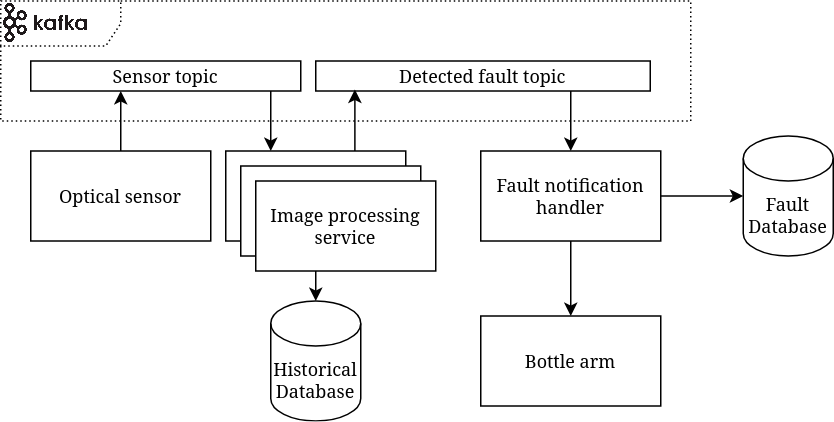
\includegraphics[scale = 0.4]{appendix/appendixA.png}
    \caption{Suggested design from original report}
    \label{fig:appendixA}
\end{figure}


\end{document}
